\documentclass{article}
\usepackage{amsmath}
\usepackage{amssymb}
\usepackage[a4paper, top=25mm, bottom=25mm, left=25mm, right=25mm]{geometry}
\usepackage{pgfplots}
\usepackage{mathtools}
\usepgfplotslibrary{fillbetween}
\pgfplotsset{compat=1.18}

\begin{document}
\pagestyle{empty}
\large

\begin{center}
2024-2025 Fall \\MAT123-02,05 Final\\(09/01/2025)
\end{center}

\noindent 1. Evaluate the following integrals.

\hfill

\noindent (a) $\displaystyle\int\frac{dx}{2\cos x+3}$

\hfill

\hfill

\noindent (b) $\displaystyle\int\frac{\sqrt{5-x^2}}{x}\,dx$

\hfill

\hfill

\noindent (c) $\displaystyle\int\frac{dx}{1-x^4}$

\hfill

\hfill

\noindent (d) $\displaystyle\int\ln\left(1+x^2\right)\,dx$

\hfill

\hfill

\noindent 2. Consider the region $R$ bounded by the curves $y=x,\:y=x^2$ and $y=x^2/2$.

\hfill

\noindent (a) Find the area of the region $R$.

\hfill

\noindent (b) Write a definite integral (do not evaluate) by using the Washer Method, which gives the volume of a solid obtained by rotating the region $R$ about the $y$-axis.

\hfill

\noindent (c) Write a definite integral (do not evaluate) by using the Cylindrical Shell Method, which gives the volume of the solid obtained by rotating the region $R$ about the line $y=2$.

\hfill

\noindent 3. Use the Integral Test to determine the existence of the sum of the series $\displaystyle\sum_{n=1}^\infty n\mathrm{e}^{-n^2}$.

\hfill

\noindent 4. Determine whether the series $\displaystyle\sum_{n=1}^\infty(-1)^{n+1}\left(\frac1n\right)^{1/n}$ is convergent or divergent.

\hfill

\noindent 5. Find the Maclaurin series of $f(x)=\sqrt{\mathrm{e}^x}$ and determine the interval of convergence of this series.

\newpage

\begin{center}
2024-2025 Final (09/01/2025) Solutions\\
(Last update: 21/08/2025 00:12)
\end{center}

\noindent 1.

\hfill

\noindent (a) Use the tangent half-angle substitution, which is also called the Weierstrass substitution. Let $\displaystyle t = \tan\left(\frac x2\right)$. Then

\[\sin x={\frac{2t}{1+t^{2}}},\quad\cos x={\frac{1-t^{2}}{1+t^{2}}},\quad dx={\frac2{1+t^{2}}}\,dt\]

\[\int\frac{dx}{2\cos x+3}=\int\frac1{2\left(\dfrac{1-t^2}{1+t^2}\right)+3}\cdot\frac2{1+t^2}\,dt=\int\frac2{5+t^2}\,dt=\frac25\int\frac1{\left(1+\left(\dfrac t{\sqrt5}\right)^2\right)}\,dt\]

\hfill

\noindent Let $u=\dfrac t{\sqrt5}$, then $\sqrt5\,du=dt$.

\begin{align*}\frac25\int\frac1{\left(1+\left(\dfrac t{\sqrt5}\right)^2\right)}\,dt&=\frac{2\sqrt5}5\int\frac1{1+u^2}\,du=\frac{2\sqrt5}5\arctan u+c=\frac{2\sqrt5}5\arctan\frac t{\sqrt5}+c\\&=\boxed{\frac{2\sqrt5}5\arctan\left(\frac1{\sqrt5}\cdot\tan\left(\frac x2\right)\right)+c,\quad c\in\mathbb{R}}\end{align*}

\hfill

\hfill

\noindent (b) Let $\displaystyle x=\sqrt5\sin u$ for $\displaystyle-\frac\pi2\leq u<\frac\pi2$, then $dx=\displaystyle\sqrt5\cos u\,du$.

\begin{align*}\mathrm{I}&=\int\frac{\sqrt{5-x^2}}{x}\,dx=\int\frac{\sqrt{5-5\sin^2u}}{\sqrt5\sin u}\cdot\sqrt5\cos u\,du\qquad\left[\sin^2u+\cos^2u=1\right]\\\\&=\sqrt5\int\sqrt{\cos^2u}\cot u\,du\qquad\left[\cos u>0\right]\\\\&=\sqrt5\int\cos u\cdot\cot u\,du=\sqrt5\int\frac{\cos^2u}{\sin u}\,du=\sqrt5\int\frac{1-\sin^2u}{\sin u}\,du\\\\&=\sqrt5\int\left(\csc u-\sin u\right)\,du=\sqrt5\left(-\ln\left|\cot u+\csc u\right|+\cos u\right)+c\end{align*}

\hfill

\noindent Recall that $\displaystyle x=\sqrt5\sin u$.

\[\sin u=\frac x{\sqrt5}\implies\sin^2u=\frac{x^2}5\implies\cos^2 u=\frac{5-x^2}5\implies\cos u=\frac{\sqrt{5-x^2}}{\sqrt5}\]

\[\cot u=\frac{\cos u}{\sin u}=\frac{\sqrt{5-x^2}}x,\qquad\csc u=\frac1{\sin u}=\frac{\sqrt5}x\]

\hfill

\noindent Therefore,
\[\mathrm{I}=\boxed{-\sqrt5\ln\left|\frac{\sqrt{5-x^2}}x+\frac{\sqrt5}x\right|+\sqrt{5-x^2}+c,\quad c\in\mathbb{R}}\]

\hfill

\noindent (c) Use partial fractions to compute the integral.

\begin{align*}\mathrm{I}&=\int\frac1{1-x^4}\,dx=\int\frac1{\left(1-x^2\right)\left(1+x^2\right)}\,dx=\int\frac1{(1-x)(1+x)\left(1+x^2\right)}\,dx\\\\&=\int\left(\frac A{1-x}+\frac B{1+x}+\frac{Cx+D}{1+x^2}\right)\,dx\end{align*}

\hfill

\[\begin{array}{c}
A(1+x)\left(1+x^2\right)+B(1-x)\left(1+x^2\right)+(Cx+D)(1+x)(1-x)=1\\
x^3(A-B-C)+x^2\left(A+B-D\right)+x\left(A-B+C\right)+A+B+D=1
\end{array}\]

\hfill

\noindent Equate the coefficients of like terms.

\[\left.\begin{array}{rc}
A-B-C=0&(1)\\
A+B-D=0&(2)\\
A-B+C=0&(3)\\
A+B+D=1&(4)
\end{array}\right\}\quad\begin{array}{c}
(1)\:\&\:(3)\rightarrow2A-2B=0\\
(2)\:\&\:(4)\rightarrow2A+2B=1\\[1em]
\therefore A=\dfrac14,\quad B=\dfrac14\\[1em]
(1)\rightarrow C=0,\quad (2)\rightarrow D=\dfrac12
\end{array}\]

\noindent Rewrite the integral.

\begin{align*}\mathrm{I}&=\int\left(\frac A{1-x}+\frac B{1+x}+\frac{Cx+D}{1+x^2}\right)\,dx=\int\left(\frac1{4(1-x)}+\frac1{4(1+x)}+\frac1{2\left(1+x^2\right)}\right)\,dx\\\\&=\boxed{-\frac14\ln|1-x|+\frac14\ln|1+x|+\frac12\arctan\left(x\right)+c,\: c\in\mathbb{R}}\end{align*}

\hfill

\noindent (d) Use the method of integration by parts.

\[\left.\begin{array}{cc}
u=\ln\left(1+x^2\right) \implies du=\dfrac{2x}{1+x^2}\,dx\\[1em]
dv=dx\implies v=x
\end{array}\right\}\rightarrow \int u\,dv=uv-\int v\,du\]
\begin{align*}\int\ln\left(1+x^2\right)\,dx&=x\ln\left(1+x^2\right)-\int\frac{2x^2}{1+x^2}\,dx=x\ln\left(1+x^2\right)-\int\frac{2x^2+2-2}{1+x^2}\,dx\\\\&=x\ln\left(1+x^2\right)-2\int dx+2\int\frac{\,dx}{1+x^2}\\\\&=\boxed{x\ln\left(1+x^2\right)-2x+2\arctan x+c,\quad c\in\mathbb{R}}\end{align*}

\newpage

\noindent 2.
\begin{center}
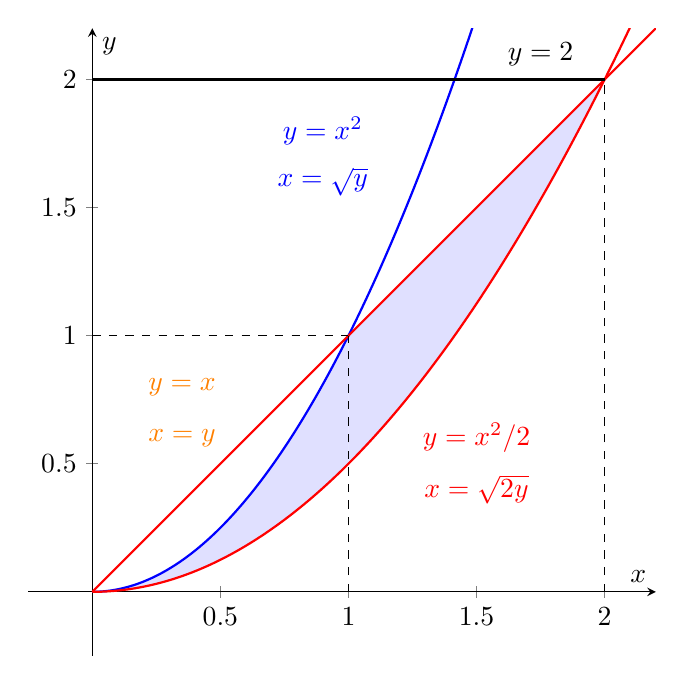
\begin{tikzpicture}
  \begin{axis}[
      axis lines=center,
      axis equal image,
      xlabel={$x$},
      ylabel={$y$},
      xmin=-0.25, xmax=2.2,
      ymin=-0.25, ymax=2.2,
      samples=250,
      clip=true,
      scale=1.4,
      domain=0:2.2,
    ]

    \addplot [thick, blue, name path=A] {x^2};
    \addplot [thick, red, name path=B] {x^2/2};
    \addplot [thick, red, name path=C] {x};
    \addplot [draw=none, name path=D] {0};
    \addplot [blue!20, fill opacity=0.6] fill between[of=A and B, soft clip={domain=0:1}];
    \addplot [blue!20, fill opacity=0.6] fill between[of=B and C, soft clip={domain=1:2}];
    
    \node[blue] at (0.9,1.8) {$y=x^2$};
    \node[red] at (1.5,0.6) {$y=x^2/2$};
    \node[orange] at (0.35,0.8) {$y=x$};
    \node at (1.75,2.1) {$y=2$};
    
    \node[blue] at (0.9,1.6) {$x=\sqrt y$};
    \node[red] at (1.5,0.4) {$x=\sqrt{2y}$};
    \node[orange] at (0.35,0.6) {$x=y$};
    
    \draw[dashed] (1,0)--(1,1); \draw[dashed] (0,1)--(1,1);
    \draw[dashed] (2,0)--(2,2); \draw[thick] (0,2)--(2,2);

  \end{axis}
\end{tikzpicture}
\end{center}

\noindent (a)
\begin{align*}A&=\int_0^1\left(x^2-\frac{x^2}2\right)\,dx+\int_1^2\left(x-\frac{x^2}2\right)\,dx=\left[\frac{x^3}3-\frac{x^3}6\right]_0^1+\left[\frac{x^2}2-\frac{x^3}6\right]_1^2\\\\&=\left[\left(\frac13-\frac16\right)-0\right]+\left[\left(2-\frac86\right)-\left(\frac12-\frac16\right)\right]=\boxed{\frac12}\end{align*}

\noindent (b)
\[V=\int_D\pi\left[r_2^2(y)-r_1^2(y)\right]\,dy=\boxed{\int_0^1\pi\left[\left(\sqrt{2y}\right)^2-\left(\sqrt y\right)^2\right]\,dy+\int_1^2\pi\left[\left(\sqrt{2y}\right)^2-y^2\right]\,dy}\]

\noindent (c)
\[V=\int_D2\pi\cdot h(y)\cdot r(y)\,dy=\boxed{\int_0^12\pi(2-y)\left(\sqrt{2y}-\sqrt{y}\right)dy+\int_1^22\pi(2-y)\left(\sqrt{2y}-y\right)dy}\]

\hfill

\noindent 3. Take $f(x)=x\mathrm{e}^{-x^2}$. $f$ is continuous because the product of a polynomial and an exponential expression is still continuous. $f$ is positive and decreasing for $x\geq1$. Verify the monotonicity of $f$ by taking the first derivative.

\[\frac{df}{dx}=1\cdot\mathrm{e}^{-x^2}+x\mathrm{e}^{-x^2}\cdot(-2x)=\mathrm{e}^{-x^2}\left(1-2x^2\right)\]

\[f'(x)<0\quad\text{for}\quad x>\frac{\sqrt2}2\implies f'(x)<0\quad\text{for}\quad x\geq1\]

\hfill

\noindent We may now apply the Integral Test. Take the limit for the improper integral.

\[\int_1^{\infty}x\mathrm{e}^{-x^2}\,dx=\lim_{R\to\infty}\int_1^Rx\mathrm{e}^{-x^2}\,dx=\lim_{R\to\infty}-\frac12\mathrm{e}^{-x^2}\Bigg|_1^R=\lim_{R\to\infty}-\frac12\left(\mathrm{e}^{-R^2}-\mathrm{e^{-1}}\right)=\frac1{2\mathrm{e}}\]

\hfill

\noindent The integral converges. Then the series $\displaystyle\sum_{n=1}^{\infty}n\mathrm{e}^{-n^2}$ also converges.

\hfill

\noindent 4. Apply the $n$th Term Test for the non-alternating part. Let $L$ be the value of the limit.

\[L=\lim_{n\to\infty}\left(\frac1n\right)^{1/n}\implies\ln(L)=\ln\left[\lim_{n\to\infty}\left(\frac1n\right)^{1/n}\right]\]

\hfill

\noindent We can also take the limit inside the function because $\ln$ is continuous on its domain.

\begin{align*}\ln(L)&=\lim_{n\to\infty}\ln\left[\left(\frac1n\right)^{1/n}\right]=\lim_{n\to\infty}\frac{\ln\left(\frac1n\right)}{n}\end{align*}

\hfill

\noindent To be able to use L'Hôpital's rule, take the corresponding function $f(x)=\dfrac{\ln\left(\frac1x\right)}x$.

\[\lim_{x\to\infty}\frac{\ln\left(\frac1x\right)}x\overset{\text{L'H.}}{=}\lim_{x\to\infty}\frac{x\cdot\left(-\frac1{x^2}\right)}1=\lim_{x\to\infty}-\frac1x=0\implies \ln(L)=0\implies L=1\]

\hfill

\noindent The limit $\displaystyle\lim_{n\to\infty}(-1)^{n+1}$ does not exist because of the oscillation. So, $\displaystyle\lim_{n\to\infty}(-1)^{n+1}\left(\frac1n\right)^{1/n}$ does not exist as well. Therefore, by the $n$th Term Test for divergence, the series $\displaystyle\sum_{n=1}^{\infty}(-1)^{n+1}\left(\frac1n\right)^{1/n}$ is divergent.

\hfill

\hfill

\noindent 5. The Maclaurin series of $f$ is given by $\sum_{k=0}^{\infty}\frac{f^{(k)}(0)}{k!}x^k$.

\hfill

\noindent Find $f(0),\:f'(0),\:f''(0),\:f'''(0)$ to look for the pattern.

\[f'(x)=\frac1{2\sqrt{\mathrm{e}^x}}\cdot\mathrm{e}^x=\frac12\sqrt{\mathrm{e}^x},\quad f''(x)=\frac1{4\sqrt{\mathrm{e}^x}}\cdot\mathrm{e}^x=\frac14\sqrt{\mathrm{e}^x},\quad f'''(x)=\frac1{8\sqrt{\mathrm{e}^x}}\cdot\mathrm{e}^x=\frac18\sqrt{\mathrm{e}^x}\]

\[f(0)=1,\quad f'(0)=\frac12,\quad f''(0)=\frac14,\quad f'''(0)=\frac18\]

\hfill

\noindent Therefore, $f^{(k)}(0)=\left(\dfrac12\right)^k$. Rewrite the summation formula.

\[\sum_{k=0}^{\infty}\frac{f^{(k)}(0)}{k!}x^k=\sum_{k=0}^{\infty}\frac{\left(\dfrac12\right)^k\cdot x^k}{k!}=\boxed{\sum_{k=0}^{\infty}\frac{x^k}{2^k\cdot k!}=1+\frac{x}2+\frac{x^2}8+\frac{x^3}{48}+...}\]

\hfill

\noindent Find the interval of convergence by applying the Ratio Test.

\[\lim_{k\to\infty}\left|\frac{x^{k+1}}{2^{k+1}\cdot\left(k+1\right)!}\cdot\frac{2^k\cdot k!}{x^k}\right|=\lim_{k\to\infty}\frac{x}{2k}=0<1\]

\hfill

\[\boxed{\text{The series is convergent on}\:\mathbb{R}.}\]

\end{document}